% Letter Fig. 1(b): the two scales of the simulation (observation scale M vs UV cutoff N).
% Standalone TikZ source; compile with pdflatex -> ../figure8.pdf
% Style matches the Letter figures: CM fonts, banana/cgblue palette.
\documentclass[border=3pt]{standalone}
\usepackage{amssymb,amsmath}
\newcommand{\fA}{\mathfrak A}
\newcommand{\cE}{\mathcal E}
\usepackage{tikz}
\usetikzlibrary{arrows.meta}
\definecolor{banana}{HTML}{FFD932}
\definecolor{cgblue}{HTML}{007CA5}
\definecolor{spacecadet}{HTML}{0D284C}
\begin{document}
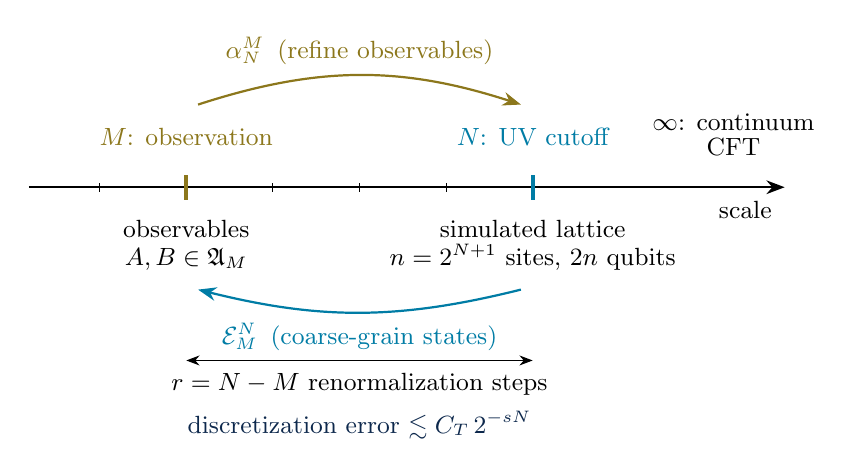
\begin{tikzpicture}[>=Stealth, font=\small]
  % ---- scale axis ----
  \draw[->, thick] (0,0) -- (9.6,0);
  \node[below] at (9.1,-0.05) {scale};
  \foreach \x in {0.9,2.0,3.1,4.2,5.3,6.4} \draw (\x,-0.06) -- (\x,0.06);
  % ---- M marker (observation) ----
  \draw[line width=1.6pt, banana!55!black] (2.0,-0.16) -- (2.0,0.16);
  \node[above, banana!55!black] at (2.0,0.40) {$M$: observation};
  \node[below, align=center] at (2.0,-0.30) {observables\\[-1pt] $A,B\in\fA_{M}$};
  % ---- N marker (UV cutoff) ----
  \draw[line width=1.6pt, cgblue] (6.4,-0.16) -- (6.4,0.16);
  \node[above, cgblue] at (6.4,0.40) {$N$: UV cutoff};
  \node[below, align=center] at (6.4,-0.30) {simulated lattice\\[-1pt] $n=2^{N+1}$ sites, $2n$ qubits};
  % ---- continuum ----
  \node[above, align=center] at (8.95,0.28) {$\infty$: continuum\\[-2pt] CFT};
  % ---- alpha arrow (observables, Heisenberg picture) ----
  \draw[->, thick, banana!55!black] (2.15,1.05) to[bend left=18]
    node[above,midway] {$\alpha^{M}_{N}$\, (refine observables)} (6.25,1.05);
  % ---- E arrow (states, Schroedinger picture) ----
  \draw[->, thick, cgblue] (6.25,-1.30) to[bend left=14]
    node[below,midway] {$\cE^{N}_{M}$\, (coarse-grain states)} (2.15,-1.30);
  % ---- RG depth + error ----
  \draw[<->, thin] (2.0,-2.20) -- (6.4,-2.20);
  \node[below] at (4.2,-2.24) {$r=N-M$ renormalization steps};
  \node[below, spacecadet] at (4.2,-2.72) {discretization error $\lesssim C_{T}\,2^{-sN}$};
\end{tikzpicture}
\end{document}
